\documentclass[11pt, a4paper, landscape]{article}
\usepackage[american, userlastpage, vertical,triangle,utf-8]{NeyDreuwSlides_Oct08}
\usepackage{multimedia}
\usepackage{bbm}

\renewcommand*{\title}{Deep Directed Generative Models}                               % main title of the work (used for \TitlePage)
\renewcommand*{\titleshort}{Generative Models}                    % short title (used for \lfoot)
\renewcommand*{\occasion}{Seminar Selected Topics in WS 2016/2017--} % (used for \TitlePage)
\renewcommand*{\occasionshort}{Selected Topics WS 2016/2017}  % short occasion title (used for \rfoot)
\renewcommand*{\date}{01.02.2017}
\renewcommand*{\author}{André Merboldt}                                     % all the authors of the work, can be long (used for \TitlePage)
\renewcommand*{\authorshort}{Merboldt, }                                        % all the authors of the work, should be short (used for \lfoot)
\renewcommand*{\email}{\url{andre.merboldt@rwth-aachen.de}}             % all email address(es) of the authors (used for \TitlePage)
\renewcommand*{\mainauthor}{André Merboldt}                                 % the author(s) who presented the work (used for \FinalPage)
\renewcommand*{\mainauthoremail}{\email}                                  % presenter mail address(es) (used for \FinalPage)
\renewcommand*{\www}{http://www-i6.informatik.rwth-aachen.de/}            % web address (used for \TitlePage _and_ \FinalPage)
\newcommand*{\keywords}{Generative Models, Deep Learning, Generative Adversarial Network, Variational autoencoder, sigmoid belief net, variational inference, reparameterization trick}      % keywords for pdf summary


% will be set into the PDF document summary
\hypersetup{
	pdftitle={\title},
	pdfsubject={\occasion},
	pdfauthor={\author},
	pdfkeywords={\keywords}
}
\newcommand\id{\ensuremath{\mathbbm{1}}}


\begin{document}

%%%%%%%%%%%%%%%%%%%%%%%%%%%%%%%%%%%%%%%%%%%%%%%%%
\TitlePage


%%%%%%%%%%%%%%%%%%%%%%%%%%%%%%%%%%%%%%%%%%%%%%%%%
\NewPage\headline{Outline}
\vfill
\begin{itemize}
  \item \hyperlink{sli:introduction}{Introduction}
  \item \hyperlink{sli:applications}{Applications}
  \item \hyperlink{sli:graphicalmodel}{Deep Directed Graphical Model}
  \item \hyperlink{sli:sbn}{Sigmoid Belief Nets}
  \item \hyperlink{sli:vae}{Variational Autoencoders}
  \begin{itemize}
    \item \hyperlink{sli:reptrick}{Reparameterization Trick}
  \end{itemize}
  \item \hyperlink{sli:gan}{Generative Adversarial Networks}
  \item \hyperlink{sli:more}{More Generative Models}
  \item \hyperlink{sli:conclusion}{Conclusion}
  \item \hyperlink{sli:references}{References}
\end{itemize}
\vfill




\NewPage\headline{Literature}
\vfill
\begin{description}
	\item [R. Neal] Connectionist learning of belief networks. {\em Elsevier 1992}.
	\begin{itemize}
		\item Introducing sigmoid belief networks
	\end{itemize}
	\item [D.P. Kingma, M. Welling] Auto-Encoding Variational Bayes. {\em ICLR 2014}.
	\begin{itemize}
		\item Variational autoencoder
	\end{itemize}
	\item [D. Rezende, S. Mohamed, D. Wierstra] Stochastic Backpropagation and Approximate Inference in Deep Generative Models. {\em ICML 2014}.
	\begin{itemize}
		\item Deep latent Gaussian model with reparameterization
	\end{itemize}
	\item [I. Goodfellow] Generative Adversarial Nets. {\em NIPS 2014}.
	\begin{itemize}
		\item Introducing generative adversarial networks
	\end{itemize}
\end{description}
\vfill

\NewPage\headline{Introduction}
\vfill
\begin{itemize}
  \item Describes how data is generated
  \item Generate data similar to samples from a dataset
  \item In comparison to discriminative models
  \begin{itemize}
    \item Learn $p(x,y)$ instead of $p(y|x)$
  \end{itemize}
  \item Maximum likelihood estimation commonly used to learn parameters
\end{itemize}
\vfill

%%%%%%%%%%%%%%%%%%%%%%%%%%%%%%%%%%%%%%%%%%%%%%%%%
\NewPage\headline{Why Generative Models: Applications}
\hypertarget{sli:why}
\vfill
\begin{itemize}
  \item Unsupervised learning
  \item Dimensionality reduction (representation learning)
  \item Exploration in reinforcement learning
	\item Generative image modeling
	\begin{itemize}
		\item Compression
		\item Super-resolution
	\end{itemize}
  \item Text-to-Speech, Text-to-Image
	\item Generate data
\end{itemize}
\vfill


%%%%%%%%%%%%%%%%%%%%%%%%%%%%%%%%%%%%%%%%%%%%%%%%%
\NewPage\headline{Deep Directed Graphical Model}
\hypertarget{sli:formal}
\vfill
\begin{minipage}[t]{0.7\linewidth}
	\begin{center}
		\begin{itemize}
			%\item Dataset $X = (x^{(1)}, x^{(2)}, \dots, x^{(n)})$
			%\item Data generation process is $x \sim p(x)$
			\item $x$ depends on latent variable $z$
			\begin{itemize}
				\item $z \sim p(z)$ and $x \sim p(x|z)$
			\end{itemize}

			\item Aspects:
			\begin{itemize}
				\item Sampling
				\begin{itemize}
					\item $x \sim p(x|z)$
				\end{itemize}
				\item Learning
				\begin{itemize}
					\item Maximize the likelihood of training data
				\end{itemize}
				\item Inference
				\begin{itemize}
					\item \emph{``Good''} values for $z$
					\item $\Rightarrow p(z|x)$
				\end{itemize}
			\end{itemize}
			%\item Our goal is to generate more $x$ by sampling from $p(x)$
		\end{itemize}
	\end{center}
		\vfill
\end{minipage}
	\begin{minipage}[t]{0.2\linewidth}
		\vfill
		\begin{center}
			\includegraphics[height=8cm]{figures/latent_model}\\
		\end{center}
		\vfill
	\end{minipage}
	\vfill

	%\NewPage\headline{Problem Setup}
	%\hypertarget{sli:problem}
	%\vfill
	%\begin{minipage}[b]{0.5\linewidth}
	%\begin{itemize}
	%\item Large dataset, possibly unlabelled
	%\begin{itemize}
	%\item $X = \{x^1, \dots, x^n\}$
	%\end{itemize}
	%\item Observations are based on latent space $z$
	%\begin{itemize}
	%\item $z \sim p(z)$
	%\item $x \sim p(x|z)$
	%\end{itemize}
	%\item Posterior distribution $p(z|x)$ is intractable
	%\end{itemize}
	%\end{minipage}
	%\vfill

	%%%%%%%%%%%%%%%%%%%%%%%%%%%%%%%%%%%%%%%%%%%%%%%%%
	%\NewPage\headline{Unsupervised Representational Learning}
	%\hypertarget{sli:rep_learning}
	%\vfill
	%\begin{itemize}
	%\item Labeled datasets are expensive and hard to obtain
	%\item High-dimensional input $\Rightarrow$ representational structure
	%% TODO: example on own slide
	%\item Example: handwritten digits
	%\begin{itemize}
	%\item $28 \times 28$ pixels as input
	%\item Want to extract representative features
	%\begin{itemize}
	%\item Digits, stroke width, digit size, $\dots$
	%\end{itemize}
	%%\item Dimensionality reduction
	%%\item Generative models can be used to perform this
	%\end{itemize}
	%\item Build model of real world
	%\begin{itemize}
	%\item Understanding of the world
	%\end{itemize}
	%\end{itemize}
	%\vfill

	%%%%%%%%%%%%%%%%%%%%%%%%%%%%%%%%%%%%%%%%%%%%%%%%%
\NewPage\headline{Sigmoid Belief Nets}
\hypertarget{sli:sbn}
\vfill
\begin{minipage}[t]{0.5\linewidth}
	\vfill
	\begin{itemize}
		\item Early generative model \cite{neal:1992}
		\item Specific form of a Bayesian network
		\item Efficient sampling
		\item Difficult to train
		\begin{itemize}
			\item Evaluation over all possible\linebreak configurations
		\end{itemize}
	\end{itemize}
\end{minipage}
\begin{minipage}[t]{.5\linewidth}
	%\begin{center}
	\vfill
		\hfill\includegraphics[height=14cm]{figures/belief_net}\\
		%\end{center}
\end{minipage}
\vfill



%%%%%%%%%%%%%%%%%%%%%%%%%%%%%%%%%%%%%%%%%%%%%%%%%
\NewPage\headline{Variational Autoencoders}
\hypertarget{sli:vae}
\vfill
\begin{itemize}
	\item Recent development
	\begin{itemize}
		\item \cite{vae:2014}
		\item \cite{dlgm:2014}
	\end{itemize}
	%\item Uses variational inference to approximate the posterior
	\item Maximizes a variational lower bound on the data likelihood
	\item Variational inference
	\begin{itemize}
		\item Used to approximate posterior $p(z|x)$
		\item Faster than Markov chain Monte Carlo (MCMC)
		\item But: not asymptotically exact
	\end{itemize}
\end{itemize}
\vfill

%%%%%%%%%%%%%%%%%%%%%%%%%%%%%%%%%%%%%%%%%%%%%%%%%
\NewPage\headline{Variational Autoencoders}
\begin{center}
	\includegraphics[height=9cm]{figures/vae_horiz}\\
\end{center}
\vfill
\begin{minipage}[b]{.5\linewidth}
	\begin{itemize}
		\item Probabilistic Encoder $q_\phi(z|x)$
		\begin{itemize}
			\item Recognition model
			\item Tries to approximate $p(z|x)$
      \item $\phi$: Parameters of encoder network
			%\item Constructs a probability distribution approximating the true posterior
		\end{itemize}
	\end{itemize}
\end{minipage}
\begin{minipage}[b]{.5\linewidth}
	\begin{center}
		\begin{itemize}
			\item Probabilistic Decoder $p_\theta(x|z)$
			\begin{itemize}
				%\item Generative model
				\item Latent $z$ $\Rightarrow$ Output $x$
				\item Reconstructs input
        \item $\theta$: Parameters of decoder network
				%\item Learning: Transform $z \sim q_\phi(z|x)$
				%\item Generation: Sample from $z$
			\end{itemize}
		\end{itemize}
	\end{center}
\end{minipage}
\vfill
%\begin{itemize}
%\end{itemize}
%\includegraphics[width=0.5\linewidth]{figures/vae}

\NewOverlay\headline{Variational Autoencoders}
\begin{center}
  \includegraphics[height=9cm]{figures/vae_horiz}\\
\end{center}
\vfill
\begin{figure}
	\begin{equation}
		\Large \mathcal{L} = \underbrace{-\mathcal{D}_{\mathrm{KL}}\big(q_\phi(z|x) \| p(z)\big)}_{\mathcal{L}_{reg}} + \underbrace{\mathbb{E}_{z \sim q_\phi(z|x)}\big[ \log p_\theta(x|z)\big]}_{\mathcal{L}_{rec}}\\
	\end{equation}
	\caption{Variational Lower Bound}
\end{figure}
\vfill
%TODO write more on objective
% and how to apply rep trick on vae, how it helps
% show manifold animation (or picture at least)
% reconstructions, generated samples
% --> maybe show mnist examples and reconstruction
% --> show mnist examples and generated samples side-by-side


\NewPage\headline{Reparameterization Trick}
\begin{minipage}[t]{.5\linewidth}
	\begin{center}
		\includegraphics[height=10cm]{figures/rep_without}\\
		without trick
		\begin{align*}
			\theta &= (\mu, \sigma)\\
			z &\sim \mathcal{N}(\mu, \sigma^2 I)\\
		\end{align*}
	\end{center}
\end{minipage}

\NewOverlay\headline{Reparameterization Trick}
\begin{minipage}[t]{.5\linewidth}
	\begin{center}
		\includegraphics[height=10cm]{figures/rep_without}\\
		without trick
		\begin{align*}
			%\medskip
			\theta &= (\mu, \sigma)\\
			z &\sim \mathcal{N}(\mu, \sigma^2 I)\\
		\end{align*}
	\end{center}
\end{minipage}
\begin{minipage}[t]{0.5\linewidth}
	\begin{center}
		\includegraphics[height=10cm]{figures/rep_with}\\
		with reparameterization
		\begin{align*}
			\epsilon &\sim \mathcal{N}(0,I)\\
			z &= \mu + \sigma \odot I\\
		\end{align*}
	\end{center}
\end{minipage}

\NewPage\headline{VAE with Reparameterization Trick}
\vfill
\includegraphics[width=\linewidth]{figures/vae_with_rep}
\vfill


\NewPage\headline{Variational Autoencoders: Samples}
\hypertarget{sli:vae_results}
\vfill
\begin{minipage}[b]{.5\linewidth}
	\begin{center}
		\includegraphics[width=0.8\linewidth]{figures/mnist_samples-crop}\\
		From original dataset
	\end{center}
\end{minipage}
\begin{minipage}[b]{.5\linewidth}
	\begin{center}
		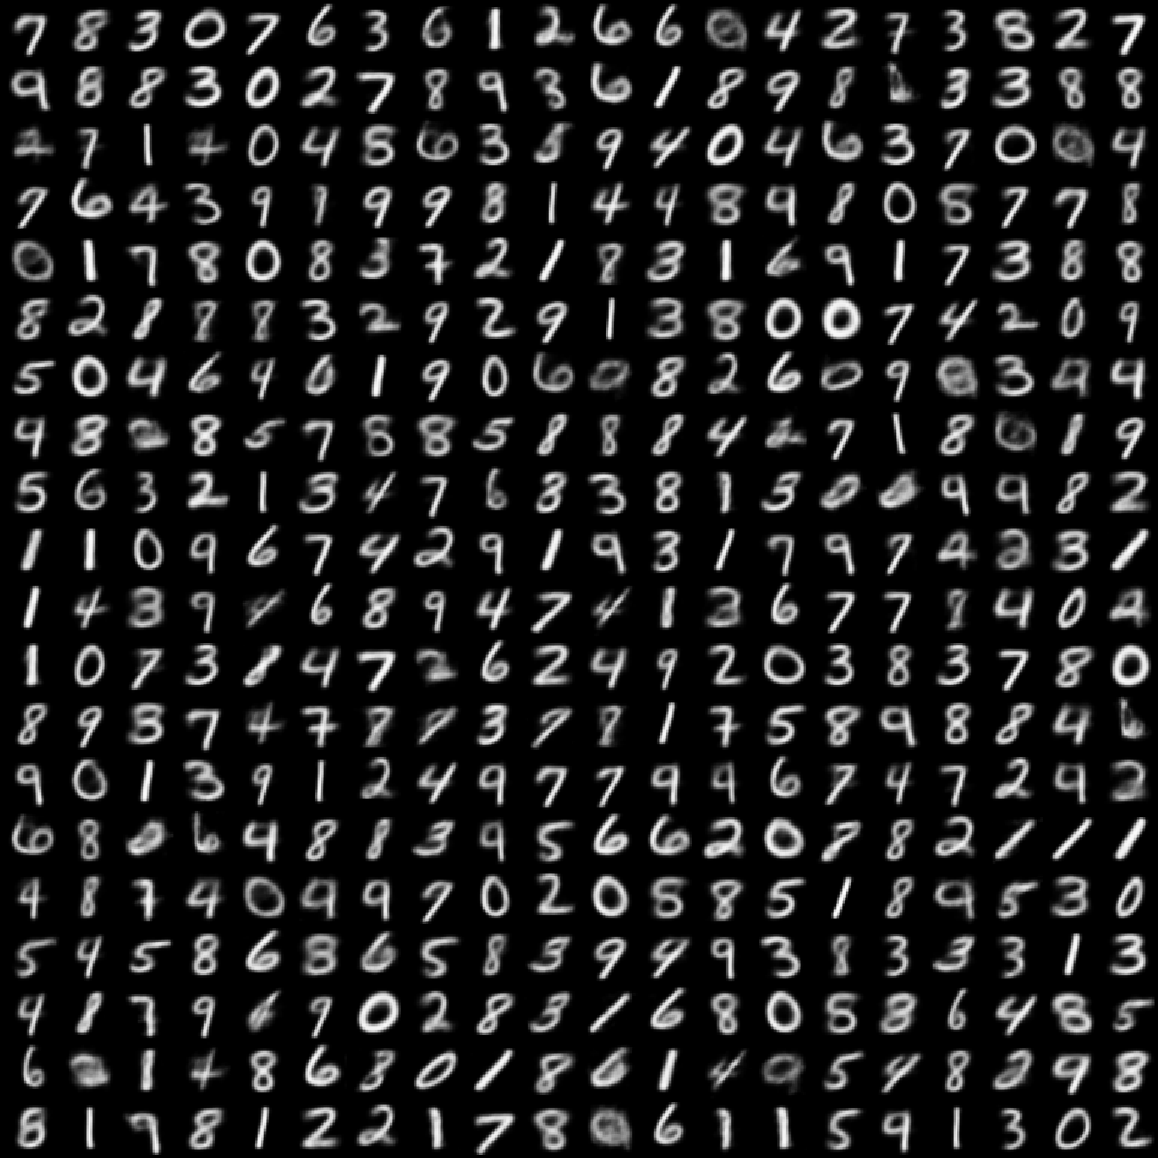
\includegraphics[width=0.8\linewidth]{figures/vae_samples}\\
		Randomly sampled
	\end{center}
\end{minipage}
\vfill
\begin{itemize}
	\item Implemented in TensorFlow \cite{tensorflow}
	\begin{itemize}
		\item \href{https://github.com/Spotlight0xff/deeplearning-seminar/tree/master/codehttp://github.com/Spotlight0xff/deeplearning-seminar}{Code here}
	\end{itemize}
	\item 50-dimensional latent space
	%\item Latent space prior: $p(z) = \mathcal{N}(0,\id)$
\end{itemize}
\vfill

\NewPage\headline{Variational Autoencoders: Reconstructions}
	\begin{center}
		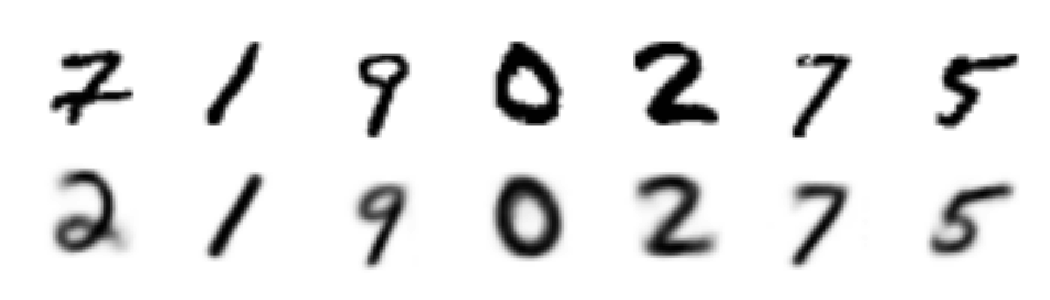
\includegraphics[width=\linewidth]{figures/reconstructions}\\
	\end{center}
	\vfill
	\begin{itemize}
    \item Fully-connected network
    \item Encoder network: 784 --- 512 --- 512 --- $(\mu, \sigma)$
    \begin{itemize}
      \item $\mu, \sigma$: 50-dimensional
    \end{itemize}
    \item Deocder network: 50 --- 512 -- 512 -- 784
    \item $p(z) = \mathcal{N}(0, I)$
	\end{itemize}
\vfill



\NewPage\headline{Variational Autoencoders: Learned Manifold}
	\begin{center}
		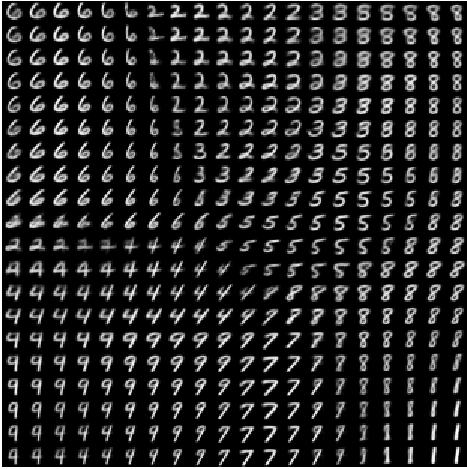
\includegraphics[width=0.5\linewidth]{figures/vae_manifold}\\
		\vfill
		Manifold plotting in 2-dimensional latent space ${[-3,3]}^2$
		\vfill
	\end{center}



	%%%%%%%%%%%%%%%%%%%%%%%%%%%%%%%%%%%%%%%%%%%%%%%%%
\NewPage\headline{Generative Adversarial Nets}
\hypertarget{sli:gan}
\vfill
\begin{itemize}
	\item Proposed in 2014 by \cite{gan:2014}
	\item Intuitive game-theoretic approach
	\item Two networks playing against each other:
	\begin{itemize}
		\item Generator $G$ tries to produce data like those in the dataset
		\item Discriminator $D$ tells fake and real data apart
	\end{itemize}
	\item Generator tries to fool the discriminator
	\item Difficult to train
	%\item Has taken off in the last year (2016)
	%\item Simple idea, but hard to train
\end{itemize}
\vfill


\NewPage\headline{Generative Adversarial Nets}
	\begin{center}
		\includegraphics[width=\linewidth]{figures/gan_conceptual}\\
	\end{center}

\NewPage\headline{Generative Adversarial Nets}
\vfill
	Objective for discriminator $D$:
	\begin{equation}
    \mathcal{L}_d = \max_{D} \log\big(\log D(x) + \log (1 - D(G(z))\big)
	\end{equation}
	Objective for generator $G$:\\
	\begin{equation}
    \mathcal{L}_g = \min_{G} \log\bigg(1 - D(G(z))\bigg)
	\end{equation}
	\vfill
	Combined value function as minimax function:\\
	\begin{equation}
		\min_{G} \max_{D} V(G,D) = \mathbb{E}_{x \sim p_{data}(x)}\big[\log \big(D(x)\big)\big] + \mathbb{E}_{z \sim p(z)}\big[\log (1 - D(G(z)))\big]
	\end{equation}
\vfill

\NewPage\headline{Generative Adversarial Nets: Training}
\vfill
	\begin{center}
		\includegraphics[width=\linewidth]{images/gan_training}\\

		Credit:\thinspace{Original GAN paper \cite{gan:2014}}
		\vfill
		\begin{itemize}
			\item[(a)] Prior to training
			\item[(b)] After training the discriminator network
			\item[(c)] After training the generator network
			\item[(d)] Nash equilibrium reached
		\end{itemize}
	\end{center}
\vfill


\NewPage\headline{Generative Adversarial Nets: Samples}
	\begin{center}
		\includegraphics[width=\linewidth]{images/bedroom_5epochs-crop}\\
		\vfill
		Credit: \cite{dcgan:2015}\\ Samples of images of bedrooms generated by a DCGAN trained on the
		LSUN dataset.
		\vfill
	\end{center}

\NewPage\headline{Generative Adversarial Nets: Latent Space Interpolation}
	\begin{center}
    \vfill
    \centering
		\includegraphics[width=0.95\linewidth]{images/bedroom_latent_interpolation}
    \vfill
    $z_1$\hfill $\longrightarrow$ \hfill $\longrightarrow$ \hfill $z_2$\\
    %\raggedleft \hspace{1cm}$\longrightarrow z_2$\\
		\vfill
    \centering
		Credit: \cite{dcgan:2015}\\
		Latent space exploration through interpolation.
		\vfill
	\end{center}

	%%%%%%%%%%%%%%%%%%%%%%%%%%%%%%%%%%%%%%%%%%%%%%%%%
\NewPage\headline{More Directed Generative Models}
\hypertarget{sli:more}
\vfill
\begin{itemize}
	\item Helmholtz machine \cite{wakesleep:1995}
	\item Generative moment matching networks \cite{gmmn:2015}
	\begin{itemize}
		\item Same idea as GANs
		\item Training using maximum mean discrepancy (MMD)
	\end{itemize}
	\item Auto-regressive networks
	\begin{itemize}
		\item Deep AutoRegressive Networks \cite{darn:2014}
		\item PixelRNN \cite{pixelrnn:2016}
		\begin{itemize}
			\item model the conditional distribution of each pixel
		\end{itemize}
	\end{itemize}
\end{itemize}
\vfill


%%%%%%%%%%%%%%%%%%%%%%%%%%%%%%%%%%%%%%%%%%%%%%%%%
\NewPage\headline{Conclusion}
\hypertarget{sli:conclusion}
\vfill
\begin{itemize}
	\item Variational autoencoders
	\begin{itemize}
		\item Inference $\Rightarrow$ optimization
	\end{itemize}
	\item Generative adversarial nets
	\begin{itemize}
    \item Game-theoretic approach
		\item Promising results
	\end{itemize}
	\item Long-term goals
	\begin{itemize}
		\item Real world sensory input
		\begin{itemize}
			\item Build compact internal representation
		\end{itemize}
		\item Reasoning, prediction, and planning
	\end{itemize}
\end{itemize}
\vfill


%%%%%%%%%%%%%%%%%%%%%%%%%%%%%%%%%%%%%%%%%%%%%%%%%
\NewPage{}
\small
\bibliographystyle{i6bibliostyle}
\bibliography{presentation}
\normalsize


%%%%%%%%%%%%%%%%%%%%%%%%%%%%%%%%%%%%%%%%%%%%%%%%%
\FinalPage

\appendix
%%%%%%%%%%%%%%%%%%%%%%%%%%%%%%%%%%%%%%%%%%%%%%%%%%%%%%%%%%%%%%%%%%%%%%%%%%%%%%%%

\NewPage\headline{\appendixname: VAE-Model for Experiments}
\vfill
\begin{itemize}
  \item MNIST: Handwritten digits 28x28 pixels
	\item \textbf{Inference network}: 784 --- 512 --- 512 --- z
	\item \textbf{Generative network}: z --- 512 --- 512 --- 784
	\item Learning rate: $10^{-3}$
  \item Batch size: 128
	\item Used rectified linear units (ReLU)
	\item Sigmoid function for output layer
\end{itemize}
\vfill

\NewPage\headline{\appendixname: More Results (2-dim latent space)}
\begin{minipage}[t]{.5\linewidth}
	\begin{center}
		\includegraphics[height=8cm]{figures/mnist_samples_close_10dim.pdf}\\
		MNIST samples
	\end{center}
\end{minipage}
\begin{minipage}[t]{.5\linewidth}
	\begin{center}
		\includegraphics[height=8cm]{figures/vae_samples_close_2dim.pdf}
		$p_\theta(x|z)$ with 2-dim. $z$
	\end{center}
\end{minipage}
	\begin{center}
		\includegraphics{figures/reconstructions_2dim}\\
		Reconstructions using VAE
	\end{center}

\NewPage\headline{\appendixname: More Results (10-dim latent space)}
\begin{minipage}[t]{.5\linewidth}
	\begin{center}
		\includegraphics[height=8cm]{figures/mnist_samples_close_10dim.pdf}\\
		MNIST samples
	\end{center}
\end{minipage}
\begin{minipage}[t]{.5\linewidth}
	\begin{center}
		\includegraphics[height=8cm]{figures/vae_samples_close_10dim.pdf}
		$p_\theta(x|z)$ with 10-dim. $z$
	\end{center}
\end{minipage}
	\begin{center}
		\includegraphics{figures/reconstructions_10dim}\\
		Reconstructions using VAE
	\end{center}

\NewPage\headline{\appendixname: Derivation of Variational Objective}
\begin{align*}
	\log p(x) &= \int_z q_\phi(z|x) \log p(x) dz
	= \int_z q_\phi(z|x) \log \frac{p_\theta(x,z)}{p_\theta(z|x)} dz\\
	&= \int_z q_\phi(z|x) \log\bigg(\frac{p_\theta(z,x)}{q_\phi(z|x)} \frac{q_\phi(z|x)}{p_\theta(z|x)}\bigg) dz\\
	&= \int_z q_\phi(z|x) \bigg(\log\frac{p_\theta(z,x)}{q_\phi(z|x)} + \log\frac{q_\phi(z|x)}{p_\theta(z|x)}\bigg) dz\\
	&= \int_z q_\phi(z|x) \log \frac{p_\theta(z,x)}{q_\phi(z|x)} dz + \int_z q_\phi(z|x) \log\frac{q_\phi(z|x)}{p_\theta(z|x)} dz\\
	&= \underbrace{\int_z q_\phi(z|x) \log \frac{p_\theta(z,x)}{q_\phi(z|x)} dz}_{= \mathcal{L}}+ \underbrace{\mathcal{D}_{\mathrm{KL}}\big(q_\phi(z|x) \| p_\theta(z|x)\big) dz}_{\geq 0}\\
\end{align*}

\NewPage\headline{\appendixname: Derivation of Variational Objective}
\begin{align*}
	\mathcal{L}
	&= \int q_\phi(z|x) \log\frac{p_\theta(z,x)}{q_\phi(z|x)} dz\\
	&= \int q_\phi(z|x) \log\frac{p(z) p_\theta(x|z)}{q_\phi(z|x)}\\
	&= \int q_\phi(z|x) \bigg(\log\frac{p(z)}{q_\phi(z|x)} + \log p_\theta(x|z)\bigg) dz\\
	&= -\int q_\phi(z|x) \log\frac{q_\phi(z|x)}{p(z)} dz + \int q_\phi(z|x) \log p_\theta(x|z) dz\\
	&= -\mathcal{D}_{\mathrm{KL}}\big(q_\phi(z|x) \| p(z)\big) + \int q_\phi(z|x) \log p_\theta(x|z) dz\\
	&= \underbrace{-\mathcal{D}_{\mathrm{KL}}\big(q_\phi(z|x) \| p(z)\big)}_{\mathcal{L}_{reg}} + \underbrace{\mathbb{E}_{z \sim q_\phi(z|x)}\big[ \log p_\theta(x|z)\big]}_{\mathcal{L}_{rec}}\\
	&= \mathcal{L}_{reg} + \mathcal{L}_{rec}
\end{align*}

\NewPage\headline{\appendixname: Quotes}
\vfill
\begin{itemize}
	\item Yann LeCun on recent and upcoming breakthroughs in deep learning:
	\begin{quote}
		``The most important one, in my opinion, is adversarial training (also called GAN for Generative Adversarial Networks).''
	\end{quote}
	\url{https://www.quora.com/What-are-some-recent-and-potentially-upcoming-breakthroughs-in-deep-learning/answer/Yann-LeCun}
	\item Ian Goodfellow on GAN convergence:
	\begin{quote}
		``In terms of theory, this is an open question.

		In terms of practice, no they don’t always converge. On small problems, they sometimes converge and sometimes don’t. On large problems, like modeling ImageNet at 128x128 resolution, I’ve never seen them converge yet.''
	\end{quote}
	\url{https://www.quora.com/Do-generative-adversarial-networks-always-converge}
\end{itemize}
	\vfill

\end{document}
